\chapter{Mathematical model} \label{ch:3}

The axis orientation that is used throughout the report is defined in the first section. The equations of motion of the vehicle can be expressed after defining the axis orientation.

\section{Axis and Force orientation}

\textcolor{red}{Goede figuur toevoegen met juiste assen, onze drone is niet symmetrisch!}


The axis orientations is chosen as a body fixed frame as depicted in Figure \ref{fig:bodyframe}. The rotation around the $X_b$ axis is called Pitch, the rotation around the $Y_b$ axis is called Roll and the rotation around the $Z_b$ axis is called Yaw. Because the drone used in this report has a slender design, will make roll control harder than pitch control.

\begin{figure}[H]
\centering
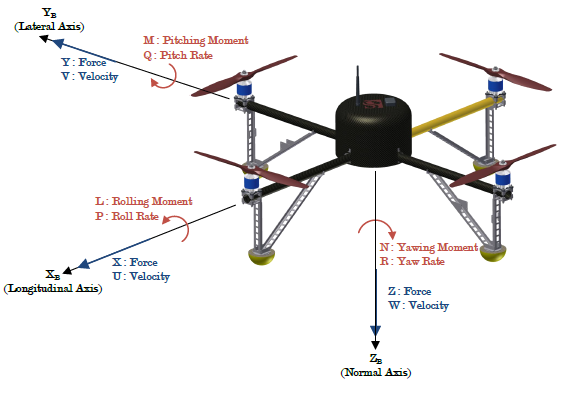
\includegraphics[width=\textwidth]{bodyframe.PNG}
\caption{Mode shapes of a pinned-sliding beam system}
\label{fig:bodyframe}
\end{figure}

Additionally, velocities,the forces and moments are also visible in Figure \ref{fig:bodyframe}. The total velocity $\bar{V}$ is defined in Equation \ref{eq:velocity}.
\begin{equation}
\bar{V}=\sqrt{U^2 +V^2+W^2}
\label{eq:velocity}
\end{equation}



\section{Kinematics}
The six degrees of freedom equations of motion for a drone are defined in Equations \ref{eq:motion1}.

\begin{equation} \label{eq:motion1}
\begin{aligned}
X=m\left(\dot{U}+WQ-VR\right)\\
Y=m\left(\dot{V}+UR-WP\right)\\
Z=m\left(\dot{W}+VP-UQ\right)\\
L=I_{xx} \dot{P}+QR \left(I_{zz} -I_{yy} \right)\\
M=I_{yy} \dot{Q}+PR \left(I_{xx} -I_{zz} \right)\\
N=I_{zz} \dot{R}+PQ \left(I_{yy} -I_{xx} \right)\\
\end{aligned}
\end{equation}

In which $I_{xx}$, $I_{yy}$ and $I_{zz}$ are the moments of inertia around the body's axis, and $m$ the mass of the vehicle.

Thereby it is assumed that: 
\begin{itemize}
\item The aircraft has a constant mass. \\
\item The aircraft is a rigid body. \\
\item $I_{xy}$ and $I_{yz}$ are zero, because of aircraft symmetry. \\
\item $I_{xz}$ is negligibly small. \\
\end{itemize}


\subsection{State-Space representation}
A state-Space respresentation is an easy way to describe the dynamics. A linear model needs to be created if the state matrices are desired to simulate the system. The Forces and moments are seen as inputs into the plant, gives as $\left[ F_x F_y F_z \tau_{\phi} \tau_{\theta} \tau_{\psi} \right]^T$. Linearization around point $x^*$ is derived if the following trigionomic assumptions are made: $sin(\alpha) \approx \alpha$,$cos(\alpha) \approx 1$ and $tan(\alpha) \approx \alpha$. Thereby is assumed that the states are small. The resulting system is visible in Equation \ref{}

\begin{equation}
\begin{aligned}
\dot{\phi} &= p + q \phi \theta +r \theta \\
\dot{\theta} &= q-r \psi  \\
\dot{\psi} &= q\phi +r \\
\dot{p} &= \frac{(I_y-I_z)}{I_x}rq + \frac{\tau_{\phi}}{Ix} \\
\dot{q} &= \frac{(I_z-I_x)}{I_y}pr + \frac{\tau_{\theta}}{I_y} \\
\dot{r} &= \frac{(I_x-I_y)}{I_z}pq + \frac{\tau_{\psi}}{I_z} \\
\dot{u} &= -qw+rv-g\theta \\
\dot{v} &= pw-ru+g\phi \\
\dot{w} &= -pv+qu+g-\frac{Fz}{m} \\
\dot{x} &= u+v(\theta \psi -\psi) + w(\phi \psi +\theta) \\
\dot{y} &= u\psi + v(\phi\theta\psi+1) + w(\psi\theta -\phi) \\
\dot{z} &= -u\theta +v\phi+w \\
\end{aligned}
\end{equation}

%\begin{equation} \label{eq:statematrices}
%A =
%\begin{bmatrix}
%0&0&0&1&0&0&0&0&0&0&0&0\\
%0&0&0&1&0&0&0&0&0&0&0&0\\
%0&0&0&1&0&0&0&0&0&0&0&0\\
%0&0&0&1&0&0&0&0&0&0&0&0\\
%0&0&0&1&0&0&0&0&0&0&0&0\\
%0&0&0&1&0&0&0&0&0&0&0&0\\
%0&0&0&1&0&0&0&0&0&0&0&0\\
%0&0&0&1&0&0&0&0&0&0&0&0\\
%0&0&0&1&0&0&0&0&0&0&0&0\\
%0&0&0&1&0&0&0&0&0&0&0&0\\
%0&0&0&1&0&0&0&0&0&0&0&0\\
%0&0&0&1&0&0&0&0&0&0&0&0
%\end{bmatrix}
%\end{equation}


\section{Forces and moments}
The forces and moments working on the vehicle can be diveded in three categories: Gravity, actuators and aerodynamics. 

\subsection{Gravity}
The gravitational force is a force that pulls an object towards the center of earth. That is why it is defined as follows in earth fixed frame in Equation \ref{eq:earthgrav}. 
\begin{equation} \label{eq:earthgrav}
\begin{bmatrix}
F_x\\
F_y\\
F_z
\end{bmatrix} = \begin{bmatrix}
0\\0\\1
\end{bmatrix} mg
\end{equation}

Since the system is defined in a body fixed frame axis, the gravitational force varies when the vehicle experiences pitch or roll rotation. This is why the forces are defined as Equation \ref{eq:Fg} with use of the euler angles transformation.

\begin{equation}
\begin{bmatrix}
X_g\\
Y_g\\
Z_g
\end{bmatrix} = \begin{bmatrix}
-sin(\theta) \\cos(\theta)sin(\phi) \\ cos(\theta) cos(\phi)
\end{bmatrix} mg
\end{equation}

\subsection{Actuator}

\textcolor{red}{Figuur toevoegen met motorvolgorde!}

The vehicle is able to hover by use of generating a thrust by the propellers attached to brushless motors. The total thrust is defined in Equation \ref{eq:thrust}.
\begin{equation}\label{eq:thrust}
Z=-\left(T_1+T_2+T_3+T_4 \right)
\end{equation}

This thrust is generated in upwards $Z_b$ direction. Moreover, the thrust also introduces several moments inside the systems, because of the propellors generating thrust outside the center of gravity. The moments on the vehicle are defined as in Equation \ref{eq:momentsthrust1} to \ref{eq:momentsthrust3}.

\begin{equation} 
\label{eq:momentsthrust1}
L=d\left(T_3+T_2-T_4-T_1)\right)
\end{equation}
\begin{equation}
M=d\left(T_2+T_4-T_1-T_3)\right)
\end{equation}
\begin{equation} \label{eq:momentsthrust3}
N = l_c 
\end{equation}

\subsection{Aerodynamics}
Due to airflow there will also occur some by-effects, for instance drag. The force that is generated by drag is defined in Equation \ref{eq:drag}. 
\begin{equation}\label{eq:drag}
F_D=\frac{1}{2} \rho C_D A\bar{V}^2
\end{equation}

In which, $F_D$ is the drag force, $\rho$ density of the medium, $C_D$ the drag constant and $A$ the front surface.\\
The forces are again transformed in the body fixed frame, leading to Equation \ref{eq:dragbff}.

\begin{equation} \label{eq:dragbff}
\begin{bmatrix}
X_D\\Y_D\\Z_D
\end{bmatrix} = 
\begin{bmatrix}
\frac{1}{2} \rho C_D A_X U^2 \\
\frac{1}{2} \rho C_D A_Y V^2 \\
\frac{1}{2} \rho C_D A_Z W^2
\end{bmatrix}
\end{equation}

\section{Parameter identification}
Certain parameters needs to be known to complete the system dynamics. Some of these parameters have to be defined by experiments i.e. Center of Gravity (CoG), mass moment of inertia and thrust profile per motor-propeller set. 

\subsection{Thrust profiles}
Seperate thrust profiles have been created to take the differences in thrust into account in the simulation. No component gives the same results, because of manufacturing uncertainties. Additionally are there some steps to generate thrust, from the output send to the motor. It goes through the ESC, which transforms the 5 Voltage input into a 22 Volts blocksignal output into the motor. Consequently will the motor transform this into a rotational speed and as a result will the aerodynamics generate a thrust via the propellers. Since these components differ from one another, the thrust outputs will vary as well. For instance ESC's from the same producer can differ $\pm 2$ $\%$ from eachother and there is some manufacturing variation in the motors and propellers as well.\\
Thereby are some measurements done to take this effects into account. All inaccuracies can be taken into account by creating a thrust-curve dependent on the $pwm$ motor output. A test setup has been created, which is depicted in Appendix Figure .... , with a loadcell to measure thrust. During the experiments, there has been taken into account that the turbulences are not or nearly affecting results.\\

\begin{figure}[H]
\centering
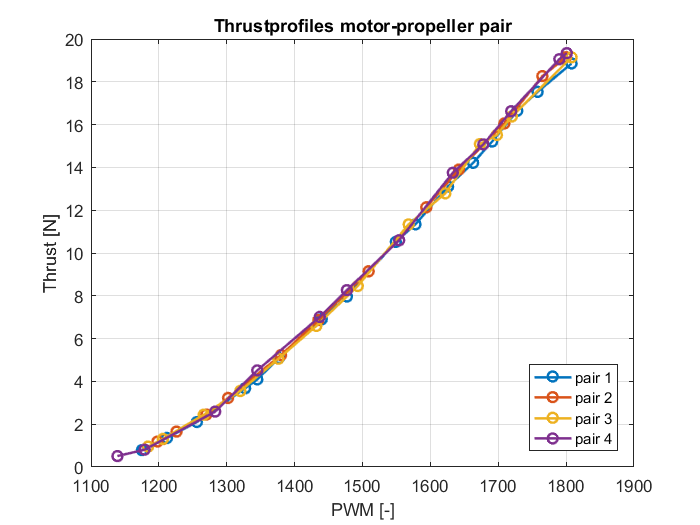
\includegraphics[width=\textwidth]{Thrustprofiles.png}
\caption{Experimental approach of defining thrust-profiles.}
\label{fig:thrustprof}
\end{figure}

The results of the thrust-profiles are depicted in Figure \ref{fig:thrustprof}. As can be seen in Figure \ref{fig:thrustprof}, the difference is almost neglictable in the area which the motors operating most of the time (1400-1600 $pwm$). At higher and lower $pwm$-values, there is some difference in thrust.\\
Additionally, the thrustprofiles show that the $PWM$ shows a linear progress, especially around hovering (1400-1550 $PWM$). This means that there does not have to take into account much nonlinear effects here.

\subsection{Center of Gravity}
The center of gravity has been defined by tethering it on the ceiling. The location in $xy$-plane has been found by getting tether it on different places on the drone and receiving a horizontal oriented drone. Furthermore this is also done to obtain the CoG in the $z$-direction. Alternetly the drone had to be tethered in a way such that the orientation of the drone would be vertical. Hence the $z$-direction would be found.\\















\subsection{Mass moment of inertia}
The mass moment of Inertia is derived with an experimental approach called a 'bifilar pendulum'. A bifilar pendulum consists of tethering the body with two parallel wires. Therefore it is allowed to rotate freely about a given axis. A small moment is applied to the body, which starts to oscillate around this axis. The moment of inertia can be determined with Equation \ref{eq:bifilar}[1].

\begin{equation}
\label{eq:bifilar}
I_{ii}=\frac{mgr^2}{4 \pi^2 L f^2}
\end{equation}

wherein $I_{ii}$ is the moment of inertia around $xx$-, $yy$- and $zz$-axis, $m$ the mass of the body, $g$ is gravitational acceleration, $r$ is the distance from CoG to wire-body connection, $L$ length of the wire and $f$ the frequency of oscillating equal to $f=2\pi \omega$. This means that the only variable will be the frequency, which can be measured by the oscillation time $T=\frac{1}{f}$. To get more accurate result, the oscillation is mearured $n$ times, and thereby be averaged. The results of the experiments are depicted in Table \ref{tab:inertia}.\\

\begin{table}[H]
\centering
\caption{Moments of inertia}
\label{tab:inertia}
\begin{tabular}{|l|l|} \hline
         & I $\left[kg \cdot m^2\right]$ \\ \hline
$I_{xx}$ & 0.025028 \\ \hline
$I_{yy}$ & 0.16196 \\ \hline
$I_{zz}$ & 0.17079 \\ \hline
\end{tabular}
\end{table}

Hereby has been taken into account that the off-diagonal terms are zero. This is because the $I_{xy}$ and $I_{yx}$ are zero because of symmetry. The same accounts for $I_{xz}$ and $I_{zx}$. Thereby is $I_{yz}$ and $I{zy}$ is neglitably small.\\\\

\textcolor{red}{add pictures of the test setup in appendix and derive the equation}\\

\url{https://conservancy.umn.edu/bitstream/handle/11299/182514/Habeck_UROP%20Final%20Report.pdf?sequence=3&isAllowed=y}\\
















